\documentclass{article}
\usepackage[utf8]{inputenc}
\usepackage{amsmath, amssymb, amsthm}
\usepackage[margin=1in]{geometry}
\usepackage{graphicx}  % For including images
\usepackage{listings}  % For including code
\usepackage{xcolor}  % For code highlighting
\usepackage{subcaption}  % For subfigures
\usepackage{hyperref}
\usepackage{tikz}
\usepackage{pdfpages}
\usetikzlibrary{positioning}

% Define theorem environments
\newtheorem{theorem}{Theorem}
\newtheorem{lemma}{Lemma}
\newtheorem{definition}{Definition}
\newtheorem{corollary}{Corollary}
% Define custom solution environment
\newenvironment{solution}{\noindent\textbf{Solution:} }{\qed}
% Code listing style
\lstset{
    language=Python,
    basicstyle=\ttfamily\footnotesize,
    keywordstyle=\color{blue},
    commentstyle=\color{gray},
    stringstyle=\color{red},
    breaklines=true,
    numbers=left,
    numberstyle=\tiny\color{gray},
    frame=single
}
\usetikzlibrary{positioning, shapes, arrows.meta}

\title{ECE-GY 7143 Introduction to Deep Learning \\ \Large Homework 3}
\author{Ali Hamza (ah7072)}
\date{\today}

\begin{document}
\maketitle

\section*{Problem 1}
We are given the function $f(x, y) = 4x^2 - 4y^2$. We want to solve the minimax optimization problem $\min_x \max_y f(x, y)$.

\paragraph{a. Determine the saddle point of this function.}

A saddle point $(x^*, y^*)$ is a critical point where the gradient is zero, $\nabla f(x^*, y^*) = (0, 0)$, and the Hessian matrix has both positive and negative eigenvalues First, we compute the gradient of $f(x, y)$:
$$ \nabla f(x, y) = \left( \frac{\partial f}{\partial x}, \frac{\partial f}{\partial y} \right) $$
$$ \frac{\partial f}{\partial x} = \frac{\partial}{\partial x}(4x^2 - 4y^2) = 8x $$
$$ \frac{\partial f}{\partial y} = \frac{\partial}{\partial y}(4x^2 - 4y^2) = -8y $$
To find critical points, we set the gradient components to zero:
$$ 8x = 0 \implies x = 0 $$
$$ -8y = 0 \implies y = 0 $$
The only critical point is $(0, 0)$. Next, we compute the Hessian matrix to classify the critical point:
$$ H(x, y) = \begin{pmatrix} \frac{\partial^2 f}{\partial x^2} & \frac{\partial^2 f}{\partial x \partial y} \\ \frac{\partial^2 f}{\partial y \partial x} & \frac{\partial^2 f}{\partial y^2} \end{pmatrix} $$
$$ \frac{\partial^2 f}{\partial x^2} = \frac{\partial}{\partial x}(8x) = 8 $$
$$ \frac{\partial^2 f}{\partial y^2} = \frac{\partial}{\partial y}(-8y) = -8 $$
$$ \frac{\partial^2 f}{\partial x \partial y} = \frac{\partial}{\partial y}(8x) = 0 $$
$$ \frac{\partial^2 f}{\partial y \partial x} = \frac{\partial}{\partial x}(-8y) = 0 $$
The Hessian matrix is:
$$ H(x, y) = \begin{pmatrix} 8 & 0 \\ 0 & -8 \end{pmatrix} $$
At the critical point $(0, 0)$, the Hessian is $H(0, 0) = \begin{pmatrix} 8 & 0 \\ 0 & -8 \end{pmatrix}$. The eigenvalues of this matrix are $\lambda_1 = 8$ and $\lambda_2 = -8$. Since the eigenvalues have different signs (one positive and one negative), the critical point $(0, 0)$ is a saddle point. The function has a local minimum along the x-direction and a local maximum along the y-direction at $(0, 0)$. Thus, the saddle point is $(x^*, y^*) = (0, 0)$.


\paragraph{b. Write down the gradient descent/ascent equations for solving this problem starting at some arbitrary initialization $(x_0, y_0)$.}

For a minimax problem $\min_x \max_y f(x, y)$, we perform gradient descent on $x$ (to minimize) and gradient ascent on $y$ (to maximize).
The update rule for $x$ (gradient descent) with step size $\eta_x$ is:
$$ x_{k+1} = x_k - \eta_x \frac{\partial f}{\partial x}(x_k, y_k) $$
The update rule for $y$ (gradient ascent) with step size $\eta_y$ is:
$$ y_{k+1} = y_k + \eta_y \frac{\partial f}{\partial y}(x_k, y_k) $$
Substituting the partial derivatives we found in part a:
$$ x_{k+1} = x_k - \eta_x (8x_k) = (1 - 8\eta_x)x_k $$
$$ y_{k+1} = y_k + \eta_y (-8y_k) = (1 - 8\eta_y)y_k $$
These are the gradient descent/ascent update equations. We can use a single step size $\eta = \eta_x = \eta_y$ for simplicity:
$$ x_{k+1} = (1 - 8\eta)x_k $$
$$ y_{k+1} = (1 - 8\eta)y_k $$

\paragraph{c. Determine the range of allowable step sizes to ensure that gradient descent/ascent converges.}

Convergence to the saddle point $(0, 0)$ means that $x_k \to 0$ and $y_k \to 0$ as $k \to \infty$.
The update equations are linear recurrence relations:
$$x_k = (1 - 8\eta_x)^k x_0 \qquad y_k = (1 - 8\eta_y)^k y_0$$
For $x_k$ to converge to 0 for any initial $x_0$, we need the magnitude of the factor $(1 - 8\eta_x)$ to be less than 1:
$$ |1 - 8\eta_x| < 1 \Rightarrow -1 < 1 - 8\eta_x < 1 $$
Solving for $\eta_x$:
$$ -2 < -8\eta_x < 0 $$
$$ \frac{-2}{-8} > \eta_x > \frac{0}{-8} $$
$$ \frac{1}{4} > \eta_x > 0 \Rightarrow 0 < \eta_x < 1/4$$
$\hfill \therefore 0 < \eta_x < 1/4$

\noindent Similarly, for $y_k$ to converge to 0 for any initial $y_0$, we need:
$$ |1 - 8\eta_y| < 1 $$
This gives the same condition:
$$ 0 < \eta_y < 1/4 $$
$\hfill \therefore 0 < \eta_y < 1/4$

\noindent For convergence of both $x_k$ and $y_k$ to the saddle point, both conditions must hold. The range of allowable step sizes is $0 < \eta_x < 1/4$ and $0 < \eta_y < 1/4$.
If a single step size $\eta = \eta_x = \eta_y$ is used, the range is $0 < \eta < 1/4$.

\paragraph{d. Regular gradient descent on both variables}

Regular gradient descent attempts to find a minimum of the function $f(x, y)$. The update rule is to move in the negative gradient direction for both variables:

\[
x_{k+1}=x_k-8\eta\,x_k=(1-8\eta)x_k,\qquad
y_{k+1}=y_k-(-8\eta\,y_k)=(1+8\eta)y_k .
\]

\[
x_k=(1-8\eta)^k x_0,\qquad y_k=(1+8\eta)^k y_0 .
\]

Convergence:
\[
|1-8\eta|<1 \;\Longrightarrow\; 0<\eta<\tfrac14,\qquad
|1+8\eta|<1 \;\Longrightarrow\; -\tfrac14<\eta<0 .
\]
These two required ranges for $\eta$ ($0 < \eta < 1/4$ and $-1/4 < \eta < 0$) are contradictory. There is no positive step size $\eta > 0$ for which regular gradient descent guarantees convergence to $(0, 0)$ for arbitrary initial points $(x_0, y_0)$.
Special cases:
\begin{itemize}
  \item \((x_0,y_0)=(0,0)\): stays at the saddle.
  \item \(y_0=0\) and \(0<\eta<\tfrac14\): \(y_k=0\) and \(x_k\to0\).
\end{itemize}
In summary, regular gradient descent generally fails to find the saddle point because it treats the problem as a minimization for all variables. It tries to move towards a minimum, but the saddle point is a maximum in some directions. The minimax formulation explicitly accounts for the different objectives for different variables (minimize $x$, maximize $y$), leading to the gradient ascent update for $y$, which is crucial for convergence to the saddle point in this example.

\section*{Problem 2}

The code for this problem is in attached below.

\paragraph{a.} \textit{Train three distinct CLIP models using any combination of vision encoders (e.g. ResNet-18, ResNet-32, or ResNet-50) and text encoder (e.g. DistilBERT, BERT, or RoBERTa).}

The original code snippet provided a basic structure for a CLIP model and a single training/evaluation flow. We have refactored the code to allow for training and evaluating multiple CLIP models with different combinations of image and text encoders. The following changes were made:

\begin{enumerate}
    \item \textbf{Generalized Encoder Selection:} The \texttt{ImageEncoder} and \texttt{TextEncoder} classes were designed to be initialized with specific model names (e.g., \texttt{'resnet18'}, \texttt{'bert-base-uncased'}). The \texttt{TextEncoder} class now uses \texttt{transformers.AutoModel} for this purpose.
    \item \textbf{Refactored Training Process:} A function \texttt{train\_clip\_model} is created to encapsulate the instantiation and training loop for a single model configuration.
    \item \textbf{Configuration List for Multiple Models:} A list \texttt{model\_configurations} is introduced to easily define the specific combinations of image encoder, text encoder, expected embedding dimensions, and save file paths for the three models to be trained. For our case, we have three configurations: \texttt{   (resnet18, distilbert-base-uncased)}, \texttt{(resnet34 , bert-base-uncased)}, and \texttt{(resnet50, roberta-base)}.
    \item \textbf{Refactored Evaluation Process:} Functions \texttt{get\_image\_embeddings} and \texttt{find\_matches} are adapted. \texttt{get\_image\_embeddings} loads a specific trained model file and computes embeddings for the validation set. \texttt{find\_matches} takes a loaded model, pre-computed image embeddings, and a text query to perform and display retrieval results.
\end{enumerate}

These changes transform the original basic script into a structured notebook capable of training and evaluating multiple CLIP variations as required by the problem statement.

The three CLIP models are trained on the flickr8k dataset, which contains 8,000 images and their corresponding captions over 4 epochs as the model was seen to overfit after 4 epochs. 

\paragraph{b.} \textit{Test each of these models on two different text prompts of your choice. An example test is given at the end of the notebook above. Experiment with various prompt choices to obtain best (qualitative) results.}

The following queries were used to test the models:
\begin{enumerate}
    \item \texttt{"two friends playing basketball"}
    \item \texttt{"a boy jumping with skateboard"}
    \item \texttt{"a dog running in the grass"}
    \item \texttt{"a person riding a bike"}
    \item \texttt{"children playing outside"}
    \item \texttt{"a woman in a boat"}
    \item \texttt{"a group of people smiling"}
\end{enumerate}

These prompts were chosen to cover a range of activities and subjects, allowing us to observe how well the models can retrieve relevant images based on different contexts.

\begin{figure}[h!]
    \centering
    \begin{subfigure}{0.5\textwidth}
        \includegraphics[width=\linewidth]{images/results_distilbert-base-uncased.png}
        \caption{CLIP with ResNet-18 and DistilBERT}
    \end{subfigure}
    \begin{subfigure}{0.5\textwidth}
        \includegraphics[width=\linewidth]{images/results_bert-base-uncased.png}
        \caption{CLIP with ResNet-34 and BERT}
    \end{subfigure}
    \begin{subfigure}{0.5\textwidth}
        \includegraphics[width=\linewidth]{images/results_roberta-base.png}
        \caption{CLIP with ResNet-50 and RoBERTa}
    \end{subfigure}
    \caption{CLIP model configurations used for testing. Each model uses a different combination of image and text encoders.}
    \label{fig:clip_models}
\end{figure}

\paragraph{c.} \textit{Comment on any trends that you observe. (e.g. Does increasing scale also increase performance?) You don’t have to do rigorous tests; qualitative observations will suffice.}

\paragraph{General Observations}

All models demonstrated basic zero-shot retrieval capability, finding images broadly related to the text queries. However, none perfectly captured relational nuances (e.g., "two friends") or specific expressions ("smiling"). Occasional irrelevant outliers were retrieved by all models, indicating limitations in the learned joint embedding space, likely due to dataset size and overfitting observed during training.

\paragraph{Query-Specific Comparisons}

\begin{itemize}
    \item \textbf{'two friends playing basketball'}: All models performed similarly well on the core "basketball" concept. The Medium model showed a tennis outlier; Small and Larger did not.
    \item \textbf{'a boy jumping with skateboard'}: This query showed the clearest performance difference. The \textbf{Larger model (RN50+RoBERTa)} was best at retrieving relevant skateboard jumping images, followed by the \textbf{Medium (RN34+BERT)}, while the \textbf{Small (RN18+DistilBERT)} struggled the most. This indicates scaling helps with combining specific concepts.
    \item \textbf{'a dog running in the grass'}: All models performed comparably well, effectively finding dogs outdoors in motion.
    \item \textbf{'a person riding a bike'}: All models showed consistently excellent and comparable performance, reliably retrieving relevant cycling images.
    \item \textbf{'children playing outside'}: All models performed comparably well on this broad concept, finding diverse images of children in outdoor play.
    \item \textbf{'a woman in a boat'}: All models showed good, comparable performance, finding images of people (often women) in boats, with minor outliers.
    \item \textbf{'a group of people smiling'}: All models were fairly relevant, finding groups in contexts suggesting smiling. Capturing the specific expression was challenging for all, and the Larger model had one outlier showing a single person.
\end{itemize}

\paragraph{Trends Observed}

\begin{itemize}
    \item \textbf{Scaling Aids Concept Combination:} The most prominent trend is the improved performance on queries requiring the combination of specific concepts (like "jumping with skateboard") as model scale increases.
    \item \textbf{Modest Overall Gain from Scaling:} While specific improvements were seen, the overall qualitative performance was not drastically different across models for simpler queries.
    \item \textbf{Dataset Limitation Dominates:} The performance of all models appears significantly limited by the small size of the Flickr8k dataset relative to their capacity, leading to overfitting (as observed in training logs) and restricting their ability to generalize broadly compared to models trained on web-scale data. The benefits of larger scale are thus somewhat constrained here.
\end{itemize}

\paragraph{Conclusion}

Qualitatively, increasing model scale provided minor but noticeable improvements in image retrieval accuracy on Flickr8k, particularly for queries involving the combination of multiple concepts. However, the analysis reinforces that the dataset's scale is a primary limiting factor for generalization in these high-capacity models, leading to overfitting and tempering the performance gains from model scaling alone.

\includepdf[pages=-]{hw3q2.pdf}

\section*{Problem 3}

The code for this problem is in attached below.

\begin{figure}[h!]
    \centering
    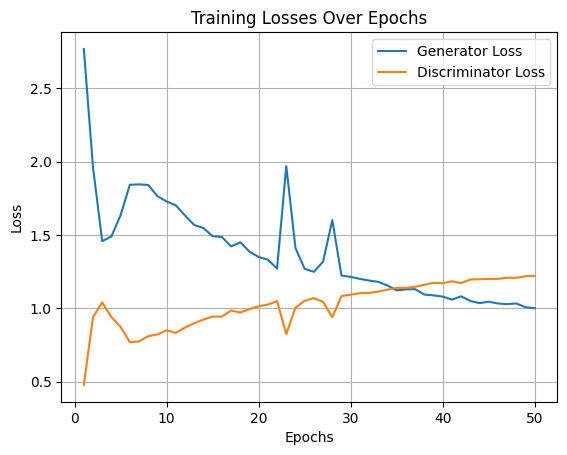
\includegraphics[width=0.8\textwidth]{images/disc_gen_loss.png}
    \caption{Training loss of the discriminator and generator over 50 epochs. The discriminator loss decreases while the generator loss increases, indicating that the generator is improving its ability to create realistic images.}
    \label{fig:clip_loss}
\end{figure}

\begin{figure}[h!]
    \centering
    \begin{subfigure}{0.19\textwidth}
        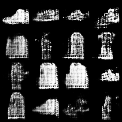
\includegraphics[width=\linewidth]{images/image_at_epoch_010.png}
        \caption{Epoch 10}
    \end{subfigure}
    \begin{subfigure}{0.19\textwidth}
        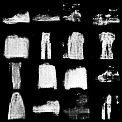
\includegraphics[width=\linewidth]{images/image_at_epoch_020.png}
        \caption{Epoch 20}
    \end{subfigure}
    \begin{subfigure}{0.19\textwidth}
        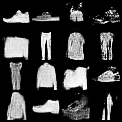
\includegraphics[width=\linewidth]{images/image_at_epoch_030.png}
        \caption{Epoch 30}
    \end{subfigure}
    \begin{subfigure}{0.19\textwidth}
        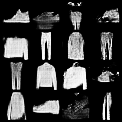
\includegraphics[width=\linewidth]{images/image_at_epoch_040.png}
        \caption{Epoch 40}
    \end{subfigure}
    \begin{subfigure}{0.19\textwidth}
        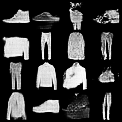
\includegraphics[width=\linewidth]{images/image_at_epoch_050.png}
        \caption{Epoch 50}
    \end{subfigure}
    \caption{Generator output at different epochs. The images show the evolution of the generated images as training progresses.}
    \label{fig:1x5_grid}
\end{figure}


In this problem, we implement and trained a Deep Convolutional GAN (DCGAN) to generate synthetic images of clothing items from the FashionMNIST dataset. The model consists of a generator network that learns to map random noise vectors to images, and a discriminator network that learns to distinguish between real FashionMNIST images and images produced by the generator. Training was performed for 50 epochs using binary cross-entropy loss and the Adam optimizer for both networks, following the specified architectures.

\subsection*{Training Loss Analysis}
Figure \ref{fig:clip_loss} illustrates the adversarial training process by showing the generator and discriminator losses over 50 epochs.
\begin{itemize}
    \item The \textbf{Discriminator Loss} starts low, as the discriminator can easily distinguish the initially poor synthetic images from real data. It then rises rapidly before beginning a general upward trend, albeit with fluctuations. A rising discriminator loss indicates that the generator is becoming more successful at producing images that the discriminator finds difficult to classify as fake, suggesting the generator is improving.
    \item The \textbf{Generator Loss} starts very high, reflecting the generator's initial inability to fool the discriminator. It drops steeply in the early epochs as the generator makes rapid progress. Throughout the remaining epochs, the generator loss continues to decrease overall but exhibits significant oscillations and spikes (e.g., around epochs 8, 23, 28). These fluctuations are characteristic of GAN training and reflect the dynamic adversarial competition between the two networks, where periods of generator improvement might be followed by the discriminator adapting, and vice versa.
\end{itemize}
The overall trend of a decreasing generator loss and an increasing discriminator loss towards the end of training suggests that the adversarial process is functional, with the generator becoming more adept at creating realistic-looking images. While the oscillations indicate some training instability, common in GANs, the final state implies the generator is producing samples that pose a notable challenge for the discriminator.

\subsection*{Generated Images}

Figure \ref{fig:1x5_grid} showcases the visual output of the generator at different stages of training. These images, generated from the same fixed set of random noise vectors, illustrate the generator's evolution:

\begin{itemize}
    \item \textbf{Epoch 10 (Figure \ref{fig:1x5_grid}(a))}: The images are primarily characterized by noise and vague, unidentifiable shapes. There is little discernible structure related to clothing items.
    \item \textbf{Epoch 20 (Figure \ref{fig:1x5_grid}(b))}: Some structure begins to emerge. Hints of forms suggestive of garments or footwear can be observed, starting to differentiate from pure noise.
    \item \textbf{Epoch 30 (Figure \ref{fig:1x5_grid}(c))}: The generated shapes are more defined and recognizable as potential clothing items (e.g., pants, shirts, shoes). However, they still appear blurry, distorted, and lack fine details.
    \item \textbf{Epoch 40 (Figure \ref{fig:1x5_grid}(d))}: Structures become clearer and more distinct. The images are more consistently identifiable as belonging to specific FashionMNIST categories, although imperfections remain.
    \item \textbf{Epoch 50 (Figure \ref{fig:1x5_grid}(e))}: By the final epoch, the generator is producing images with shapes and forms that closely resemble items from the FashionMNIST dataset. While still synthetic and not perfectly sharp, they have captured key visual characteristics of clothing items.
\end{itemize}

This visual progression demonstrates the generator's ability to leverage the adversarial feedback to gradually learn the data distribution of FashionMNIST images, successfully transitioning from generating random noise to producing increasingly realistic and structured synthetic examples over the course of training.

\includepdf[pages=-]{hw3q3.pdf}

\end{document}